\documentclass[aspectratio=169]{beamer} % 16:9 widescreen layout

\usepackage[utf8]{inputenc}
\usepackage[brazil]{babel}
\usepackage{graphicx}
\usepackage{booktabs}
\usepackage{listings}
\usepackage{tikz}
\usepackage{pgfplots}
\pgfplotsset{compat=1.18}

% --- Poli-USP Official Color Palette ---
\definecolor{PoliBlue}{RGB}{0, 70, 135}
\definecolor{USPGold}{RGB}{240, 180, 0}
\definecolor{DarkGray}{RGB}{60, 60, 60}

\usetheme{Madrid}
\usecolortheme{default}

\setbeamercolor{structure}{fg=PoliBlue}
\setbeamercolor{palette primary}{bg=PoliBlue, fg=white}
\setbeamercolor{palette secondary}{bg=PoliBlue!85!black, fg=white}
\setbeamercolor{palette tertiary}{bg=PoliBlue!70!black, fg=white}
\setbeamercolor{titlelike}{parent=palette primary, fg=white}
\setbeamercolor{block title}{bg=PoliBlue, fg=white}
\setbeamercolor{block body}{bg=PoliBlue!10!white, fg=DarkGray}
\setbeamertemplate{navigation symbols}{}

\lstset{basicstyle=\ttfamily\scriptsize, keywordstyle=\color{PoliBlue},
        columns=fullflexible, showstringspaces=false, frame=none}

\title[GCC target for educational RISC-V processor]{GCC target for educational RISC-V processor}
\subtitle{Trabalho de Conclusão de Curso}
\author[G. S. Salustiano]{Guilherme Stabach Salustiano \\ \footnotesize Orientador: Prof. Bruno de Carvalho Albertini}
\institute[PCS - EPUSP]{
    Departamento de Engenharia de Computação e Sistemas Digitais (PCS)\\
    Escola Politécnica da Universidade de São Paulo (EPUSP)
}
\date{2026}

% escala logarítmica da Figura 3 (definida no preâmbulo: '#' não sobrevive
% dentro de um frame não-fragile)
\newcommand{\lx}[1]{\plotw*ln(#1)/ln(\xmax)}

\begin{document}

% ------------------------------------------------------------------
\begin{frame}
    \titlepage
\end{frame}
% FALAR:
% - Bom dia, sou o Guilherme, orientado pelo prof. Bruno Albertini.
% - O trabalho é um backend de GCC que compila C para o processador
%   mono-ciclo do Hennessy-Patterson, o mesmo usado em PCS3225.
% - A ideia central: toda instrução que o hardware não tem, o compilador
%   sintetiza com as que ele tem.

% ------------------------------------------------------------------
\begin{frame}{Sumário}{Roteiro da apresentação}
    \tableofcontents
\end{frame}
% FALAR:
% - Contexto do processador didático, motivação e objetivo.
% - Como o GCC gera código e onde eu intervenho.
% - Um exemplo completo de síntese (XOR) e a tabela de custos.
% - Validação em quatro camadas e os resultados de custo.

% ==================================================================
\section{Contexto e Motivação}

\begin{frame}{O processador Hennessy--Patterson}{Contexto}
    \begin{columns}[T]
    \begin{column}{0.4\textwidth}
        \begin{itemize}
            \item \textit{Computer Organization and Design: RISC-V Edition} é
                  a referência em curso de arquitetura de computadores.
            \item Usado em Sistemas Digitais II (PCS3225) na Poli.
            \item Implementa um processador mono-ciclo com 8 instruções:
                  \texttt{lw sw beq add addi sub and or}
        \end{itemize}
    \end{column}
    \begin{column}{0.55\textwidth}
        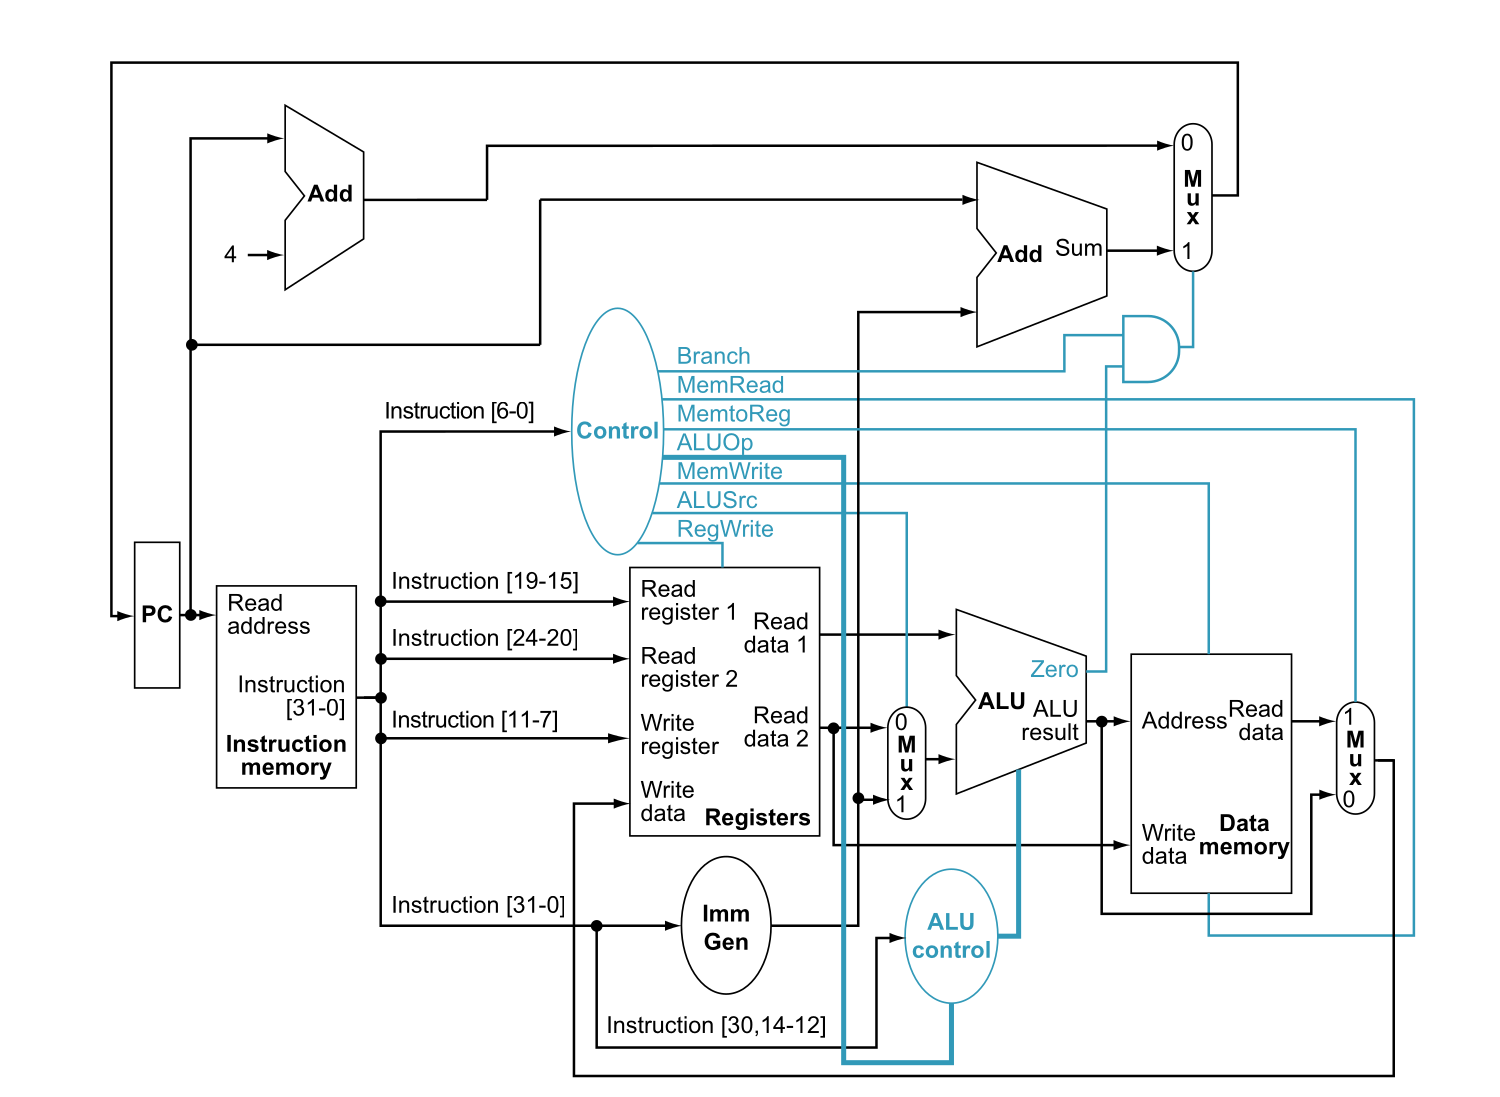
\includegraphics[width=\textwidth]{hannersy-patterson-implementation-fig4-21.png}

        \vspace{0.3em}
        \tiny Fonte: Patterson \& Hennessy, \textit{Computer Organization and
        Design: RISC-V Edition}, 2ª ed., 2020, Figura 4.21.
    \end{column}
    \end{columns}
\end{frame}
% FALAR:
% - O livro do Patterson e Hennessy é a referência do curso.
% - O aluno implementa em VHDL exatamente esse datapath (Figura 4.21).
% - São oito instruções: dois acessos a memória, um branch e cinco de ALU.
% - Não há lui, não há jalr: nem endereço grande, nem chamada de função.

\begin{frame}{Problema}{Motivação}
    \vspace{0.5em}
    {\centering\Large\color{PoliBlue}
     Não há compilador para apenas 8 instruções.\par}
    \vspace{1em}
    \begin{itemize}
        \item GCC e Clang geram no mínimo 40 instruções (RV32I).
        \item Alunos e professores precisam escrever os programas manualmente
              em assembly, limitando o tamanho dos programas.
        \item Perde-se a oportunidade de integrar o conhecimento de C do
              aluno, introduzindo a tradução e otimização de compiladores.
    \end{itemize}
\end{frame}
% FALAR:
% - O descasamento é simples: o compilador mais restrito que existe já emite
%   muito mais do que o hardware do aluno entende.
% - Então o laboratório fica preso a assembly manual e a programas de brinquedo.
% - E o elo hardware-software, que é o ponto pedagógico, não fecha.

\begin{frame}{Objetivo}
    Gerar assembly a partir de C para conjuntos de instruções
    progressivos, sintetizando toda instrução ausente com uma
    sequência equivalente no GCC.

    \vspace{1em}
    \centering\small
    \begin{tabular}{ll}
        \toprule
        \textbf{Alvo} & \textbf{ISA} \\
        \midrule
        rvsc0 & \texttt{lw sw beq add addi sub and or} \\
        rvsc1 & + \texttt{lui}, \texttt{jalr} \\
        rvsc2 & RV32I $-$ fence $-$ Zicsr \\
        rvsc3 & RV32I completo \\
        rvsc4 & RV64I \\
        rvsc5 & RV64IM \\
        rvsc6 & RV64IMFD + Zicsr \\
        rvsc7 & RV64IMAFD \\
        \bottomrule
    \end{tabular}
\end{frame}
% FALAR:
% - Oito alvos, cada um adicionando um grupo de instruções.
% - rvsc0 é exatamente o processador do livro.
% - rvsc1 acrescenta lui e jalr: é o primeiro alvo com chamada de função, ou
%   seja, o primeiro que compila um programa C de verdade.
% - Do rvsc3 em diante é RISC-V padrão; o interesse está nos dois primeiros.
% - A progressão acompanha a evolução do processador ao longo do curso.

\section{Trabalhos Relacionados}

\begin{frame}{Trabalhos relacionados}
    \begin{itemize}
        \item \textbf{Berkeley SoftFloat} — ponto flutuante em software.
        \item \textbf{MSP430}: \texttt{\_\_mspabi\_slli\_n} — shift de vários
              bits em ISA single shift.
        \item \textbf{AVR}: \texttt{\_\_mulhi3} — multiplicação em software.
    \end{itemize}
\end{frame}
% FALAR:
% - Compilar para hardware incompleto não é novo: falta FPU, falta multiplicador.
% - A saída clássica é uma função de biblioteca, o libgcc.
% - Isso não serve aqui por dois motivos: o rvsc0 não consegue nem chamar
%   função, e uma chamada esconde do aluno o custo real da instrução.
% - Por isso a síntese é feita na machine description, inline.
% - Isso eh feito via lib, n tem necessidade de mexer no codigo do compilador

% ==================================================================
\section{Desenvolvimento}

\begin{frame}{GCC Pipeline}
    \begin{center}
        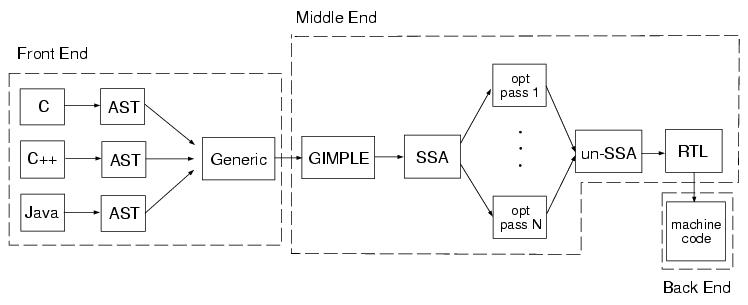
\includegraphics[width=0.9\textwidth]{gcc-internal-flow.jpg}

        \vspace{0.2em}
        \tiny Fonte: AlexeySmirnov, \textit{GNU C Compiler Internals}
        (Wikibooks), arquivo \texttt{Gcc.JPG}, CC BY-SA 3.0.
    \end{center}
\end{frame}
% FALAR:
% - Este é o pipeline do GCC, e o ponto que importa é um só: o expand.
% - O expand é o momento em que o GCC pergunta à descrição da máquina
%   "como eu faço um xor aqui?".
% - Se eu responder com três instruções em vez de uma, o xor deixa de existir.
% - Fazer no expand, e não depois, é o que garante a corretude por construção:
%   não há como um passe de otimização trazer de volta o que nunca esteve lá.

\begin{frame}[fragile]{Exemplo: XOR}
    \lstset{basicstyle=\ttfamily\normalsize}
    \large
    \textbf{Codigo}
\begin{lstlisting}[language=C]
int f(int a, int b) { return a ^ b; }
\end{lstlisting}
    \textbf{GIMPLE}
\begin{lstlisting}[language=C]
D.2418 = a ^ b;
return D.2418;
\end{lstlisting}
    \textbf{RTL}
\begin{lstlisting}[language=lisp]
(set (reg:SI 137) (xor:SI (reg:SI 135) (reg:SI 136)))
\end{lstlisting}
    \textbf{Assembly}
\begin{lstlisting}
f:
    xor  a0, a0, a1
    ret
\end{lstlisting}
\end{frame}

% FALAR:
% - Primeiro o caminho normal, com TARGET_XOR ligado.
% - O expand não faz nada: o define_insn casa direto e sai um xor.
% - Guardem o RTL do meio: é ele que muda no próximo slide.

\begin{frame}[fragile]{Exemplo: "soft" XOR}
    \lstset{basicstyle=\ttfamily\normalsize}
    \large
    \textbf{RTL}
\begin{lstlisting}[language=lisp]
(set (reg 138) (and:SI (reg 135) (reg 136)))
(set (reg 139) (ior:SI (reg 135) (reg 136)))
(set (reg 137) (minus:SI (reg 139) (reg 138)))
   (REG_EQUAL (xor:SI ...))
\end{lstlisting}
    \textbf{Assembly}
\begin{lstlisting}
f:
    and  a5, a0, a1
    or   a0, a0, a1
    sub  a0, a0, a5
    ret
\end{lstlisting}
\end{frame}
% FALAR:
% - Mesmo fonte, mesmo GIMPLE. A única diferença é a flag -mno-xor, que o
%   header do alvo injeta sozinho pelo CC1_SPEC.
% - O expand vê que xor não existe, emite a identidade e chama DONE.
% - Custo real: 3 instruções e 1 registrador extra.
% - São dois pseudo-registradores (138 e 139), não um reaproveitado: é essa
%   aresta de fluxo de dados que impede o alocador de corromper a|b.
% - O REG_EQUAL preserva a semântica para CSE e combine sem permitir que
%   nenhum deles reintroduza o xor.
% - Os dois pseudos não são detalhe estético: a versão anterior, por De Morgan,
%   reaproveitava um registrador, o IRA aliasou e o código saía errado. Foi um
%   bug real que os testes comportamentais pegaram.

\begin{frame}[fragile]{Exemplo: SLL}
    \vspace{0.5em}
    {\centering\large\color{PoliBlue}
     $\mathrm{sll}(x,0) = x$

     \vspace{0.4em}
     $\mathrm{sll}(x,n{+}1) = \mathrm{sll}(x,n) + \mathrm{sll}(x,n)$\par}
    \vspace{1.2em}

    \lstset{basicstyle=\ttfamily\normalsize}
    \large
    \begin{itemize}
        \item Se $n$ imediato:
\begin{lstlisting}
add rd, rd, rd
... # n vezes
\end{lstlisting}
        \item Se $n$ parametrizado:
\begin{lstlisting}[language=C]
for (uint32_t rd = rs1, i = 0; i < rs2; i++) rd += rd;
\end{lstlisting}
    \end{itemize}
\end{frame}
% FALAR:
% - Cada síntese vem de uma derivação algébrica, não de tentativa e erro.
% - Shift à esquerda é o caso mais limpo: por indução, é soma consigo mesmo.
% - Com contagem constante o custo é trivial e o código é reto.
% - Com contagem variável, em vez de um laço que decrementa, eu decomponho a
%   contagem em binário: cinco testes de bit cobrem qualquer valor de 0 a 31.
% - Isso derrubou o pior caso de 187 para 47 instruções.

\begin{frame}{Custo teorico}
    \centering\scriptsize
    \begin{tabular}{lrr}
        \toprule
        \textbf{Operação} & \textbf{Pior caso} & \textbf{Regs extras} \\
        \midrule
        \texttt{not}                       & 2        & 0 \\
        \texttt{xor} (reg / imm)           & 3 / 4    & 1 / 2 \\
        \texttt{ori} / \texttt{andi}       & 2        & 1 \\
        \texttt{sll} const / var           & 31 / 47  & 0 / 1 \\
        \texttt{srl} const / var           & 158 / 332 & 3 \\
        \texttt{sra} const / var           & 194 / 391 & 5 / 7 \\
        \texttt{slt} / \texttt{sltu}       & 49 / 48  & 3 / 4 \\
        \texttt{bne}                       & 3        & 1 \\
        \texttt{blt},\texttt{bltu} / \texttt{bge},\texttt{bgeu} & 16 / 17 & 7 \\
        \texttt{lb}/\texttt{lbu}           & 77 / 460 & 2 \\
        \texttt{lh}/\texttt{lhu}           & 85 / 532 & 2 \\
        \texttt{sb}                        & 32 / 95  & 3 \\
        \texttt{sh}                        & 23 / 82  & 3 \\
        \texttt{lui} (rvsc0)               & 25       & 0 \\
        \texttt{jal} (rvsc1)               & 5        & 1 \\
        \bottomrule
    \end{tabular}
\end{frame}
% FALAR:
% - Estes são números medidos, não estimados: rodo um laço com a operação e um
%   laço vazio no simulador e subtraio, então o overhead cancela exato.
% - Duas leituras importantes.
% - Primeira: o custo varia três ordens de grandeza. NOT custa 2; um load de
%   byte com endereço desconhecido custa 460.
% - Segunda: "lane conhecida" versus "desconhecida" são sequências diferentes,
%   não um intervalo. Se o compilador sabe em que byte da palavra o dado está
%   (global, variável local, campo de struct), toda a aritmética de endereço
%   some. É a otimização que mais rendeu.

% ==================================================================
\section{Validação}

\begin{frame}{Base de validação}{Metodologia}
    \begin{itemize}
        \item \textbf{rvsc0}
        \begin{itemize}
            \item 12 \textit{smoke tests} escritos à mão.
        \end{itemize}
        \item \textbf{rvsc1}
        \begin{itemize}
            \item 8 \textit{smoke tests} escritos à mão.
            \item GCC \textit{torture suite}: 1684 programas usados pelo
                  próprio GCC.
        \end{itemize}
    \end{itemize}
    \vfill
    \centering Cada teste em 5 níveis de otimização
    (\texttt{-O0} \dots{} \texttt{-Os}).
\end{frame}

\begin{frame}{Teste}{Metodologia}
    \begin{itemize}
        \item \textbf{Validação estática:} \texttt{objdump -M no-aliases} e
              checagem das operações geradas contra a lista permitida.
        \item \textbf{Validação dinâmica:} programas validados por
              \texttt{assert} no próprio código e executados no emulador
              \textbf{Spike}.
    \end{itemize}
    \vfill
\end{frame}



% FALAR:
% - A validação responde duas perguntas diferentes, e por isso são camadas.
% - "Correto por construção": nenhum mnemônico proibido saiu. Isso é estático.
% - "Correto por execução": o valor calculado é o que o C manda. Isso roda.
% - A terceira camada é o que dá escala: 1684 programas que eu não escrevi.
% - A quarta existe porque a primeira olha só o que o compilador gerou; a
%   biblioteca tinha assembly escrito à mão com instruções proibidas, e só a
%   verificação do ELF ligado pegou isso.

\begin{frame}{Torture suite test (rvsc1)}{Resultado}
    \begin{itemize}
        \item 13 testes precisaram ser pulados:
        \begin{itemize}
            \item \texttt{run\_expensive\_tests} (timeout)
            \item \texttt{c99\_runtime}
            \item \texttt{int128}
            \item \texttt{mmap} e \texttt{dfp}
        \end{itemize}
        \item \textbf{1669 testes passaram} gerando apenas as 10 instruções
              do sc1, totalizando \textbf{8345 execuções}.
    \end{itemize}
\end{frame}
% FALAR:
% - Este é o número que dá confiança no trabalho: oito mil e trezentas
%   combinações de programa e nível de otimização, zero falhas.
% - O ponto delicado é o skip: um skip pode esconder uma falha.
% - Por isso a lista de skip é derivada, não curada: eu leio a diretiva
%   dg-require do próprio teste, a mesma regra que o DejaGnu aplica.
% - E confirmei por comparação que um GCC rv32i normal falha exatamente os
%   mesmos casos, então nenhum deles é culpa da ISA restrita.
% - Zero ICE quer dizer que o compilador nunca quebrou.

% ==================================================================
\begin{frame}{Embench-IoT benchmark}{Resultado}
    \begin{itemize}
        \item Suíte livre de benchmarks para \textbf{IoT / embarcado} ---
              programas reais e pequenos, sem dependência de sistema
              operacional.
        \item \textbf{19 casos}: criptografia (\texttt{nettle-aes},
              \texttt{nettle-sha256}, \texttt{md5sum}, \texttt{crc32}),
              processamento de sinal e imagem (\texttt{edn},
              \texttt{picojpeg}, \texttt{depthconv}, \texttt{qrduino}),
              estruturas de dados e strings (\texttt{sglib-combined},
              \texttt{slre}, \texttt{wikisort}, \texttt{huffbench},
              \texttt{tarfind}), aritmética e controle
              (\texttt{aha-mont64}, \texttt{matmult-int}, \texttt{ud},
              \texttt{xgboost}, \texttt{statemate}, \texttt{nsichneu}).
        \item Duas medidas independentes: \textbf{tamanho} (\texttt{.text} a
              \texttt{-O2}) e \textbf{tempo} (instruções retiradas no Spike).
        \item Três \textit{toolchains}: \textbf{gcc17} (mesmo \textit{fork},
              \texttt{riscv32-unknown-elf}) / \textbf{rvsc2} (nativo) /
              \textbf{rvsc1} (sintetizado).
    \end{itemize}
\end{frame}

\section{Resultados}

\begin{frame}{Custo estático}{Resultados}
    \centering\tiny
    \begin{tabular}{lrrr@{\qquad}lrrr}
        \toprule
        \textbf{Benchmark} & \textbf{gcc17} & \textbf{rvsc1} & \textbf{razão} &
        \textbf{Benchmark} & \textbf{gcc17} & \textbf{rvsc1} & \textbf{razão} \\
        \midrule
        \texttt{aha-mont64} & 3.548 & 28.468 & $\times 8{,}02$ & \texttt{picojpeg} & 15.360 & 201.204 & $\times 13{,}10$ \\
        \texttt{crc32} & 380 & 1.752 & $\times 4{,}61$ & \texttt{qrduino} & 12.852 & 286.212 & $\times 22{,}27$ \\
        \texttt{depthconv} & 608 & 5.820 & $\times 9{,}57$ & \texttt{sglib-combined} & 10.824 & 34.596 & $\times 3{,}20$ \\
        \texttt{edn} & 3.244 & 59.344 & $\times 18{,}29$ & \texttt{slre} & 4.256 & 44.408 & $\times 10{,}43$ \\
        \texttt{huffbench} & 2.140 & 15.936 & $\times 7{,}45$ & \texttt{statemate} & 6.484 & 25.160 & $\times 3{,}88$ \\
        \texttt{matmult-int} & 936 & 1.500 & $\times 1{,}60$ & \texttt{tarfind} & 528 & 4.772 & $\times 9{,}04$ \\
        \texttt{md5sum} & 1.016 & 3.140 & $\times 3{,}09$ & \texttt{ud} & 1.436 & 1.964 & $\times 1{,}37$ \\
        \texttt{nettle-aes} & 4.444 & 117.652 & $\times 26{,}47$ & \texttt{wikisort} & 7.744 & 38.812 & $\times 5{,}01$ \\
        \texttt{nettle-sha256} & 6.976 & 138.472 & $\times 19{,}85$ & \texttt{xgboost} & 624 & 9.456 & $\times 15{,}15$ \\
        \texttt{nsichneu} & 19.668 & 48.548 & $\times 2{,}47$ & & & & \\
        \midrule
        \multicolumn{7}{r}{\textbf{média geométrica}} & $\mathbf{\times 6{,}99}$ \\
        \bottomrule
    \end{tabular}

    \vspace{0.6em}
    \normalsize \textbf{rvsc2 é idêntico ao gcc17 nos 19 benchmarks.}
\end{frame}
% FALAR:
% - Comparo três toolchains: o GCC upstream, o rvsc2 e o rvsc1.
% - O resultado do rvsc2 é o controle do experimento: código byte a byte igual
%   ao upstream. Ou seja, o backend em si não introduz regressão nenhuma.
% - No rvsc1 o código cresce sete vezes em média, mas a média esconde o que
%   interessa: a faixa vai de 1,4 a 26 vezes.
% - Quem paga caro é quem usa muito o que falta. AES é rotação e byte, que são
%   justamente as duas sínteses mais caras.

\begin{frame}{Custo dinâmico}{Resultado}
    \centering\tiny
    Instruções retiradas no Spike (milhões).
    \vspace{0.4em}

    \begin{tabular}{lrrr@{\qquad}lrrr}
        \toprule
        \textbf{Benchmark} & \textbf{gcc17} & \textbf{rvsc1} & \textbf{razão} &
        \textbf{Benchmark} & \textbf{gcc17} & \textbf{rvsc1} & \textbf{razão} \\
        \midrule
        \texttt{aha-mont64} & 13,0 & 196,6 & $\times 15{,}1$ & \texttt{picojpeg} & 3,6 & 108,4 & $\times 30{,}1$ \\
        \texttt{crc32} & 6,0 & 148,5 & $\times 24{,}8$ & \texttt{qrduino} & 5,1 & 159,0 & $\times 30{,}9$ \\
        \texttt{depthconv} & 54,6 & 626,3 & $\times 11{,}5$ & \texttt{sglib-combined} & 3,0 & 78,3 & $\times 26{,}0$ \\
        \texttt{edn} & 68,6 & 476,3 & $\times 6{,}9$ & \texttt{slre} & 3,0 & 43,4 & $\times 14{,}6$ \\
        \texttt{huffbench} & 2,4 & 55,9 & $\times 23{,}3$ & \texttt{statemate} & 2,1 & 12,6 & $\times 6{,}1$ \\
        \texttt{matmult-int} & 24,4 & 86,8 & $\times 3{,}6$ & \texttt{tarfind} & 5,3 & 265,9 & $\times 50{,}3$ \\
        \texttt{md5sum} & 2,9 & 20,7 & $\times 7{,}1$ & \texttt{ud} & 6,6 & 259,2 & $\times 39{,}1$ \\
        \texttt{nettle-aes} & 4,7 & 124,4 & $\times 26{,}6$ & \texttt{wikisort} & 1,6 & 10,2 & $\times 6{,}3$ \\
        \texttt{nettle-sha256} & 4,9 & 105,5 & $\times 21{,}5$ & \texttt{xgboost} & 3,8 & 225,3 & $\times 59{,}2$ \\
        \texttt{nsichneu} & 2,5 & 9,5 & $\times 3{,}8$ &  & &  \\
        \midrule
        \multicolumn{7}{r}{\textbf{média geométrica}} & $\mathbf{\times 15{,}8}$ \\
        \bottomrule
    \end{tabular}

    \vspace{0.6em}
    \normalsize \textbf{Todos os 19 benchmarks executam corretamente.}
\end{frame}

\begin{frame}{Custo estático x dinâmico}{Resultado}
    \centering
    \begin{tikzpicture}
    \begin{axis}[
        width=0.78\textwidth, height=0.62\textheight,
        xlabel={razão de tamanho (rvsc1 / gcc17)},
        ylabel={razão de tempo (rvsc1 / gcc17)},
        xmode=log, ymode=log, grid=both,
        xmin=1, xmax=40, ymin=2.5, ymax=90,
        label style={font=\small}, tick label style={font=\footnotesize},
    ]
    \addplot[only marks, mark=*, mark size=1.6pt, PoliBlue] coordinates {
        (8.02,15.1) (4.61,24.8) (9.57,11.5) (18.29,6.9) (7.45,23.3)
        (1.60,3.6) (3.09,7.1) (26.47,26.6) (19.85,21.5) (2.47,3.8)
        (13.10,30.1) (22.27,30.9) (3.20,26.0) (10.43,14.6) (3.88,6.1)
        (9.04,50.3) (1.37,39.1) (5.01,6.3) (15.15,59.2)
    };
    \addplot[dashed, gray, domain=1:40, samples=2] {x};
    \node[font=\tiny, anchor=west] at (axis cs:1.37,39.1) {\texttt{ud}};
    \node[font=\tiny, anchor=east] at (axis cs:15.15,59.2) {\texttt{xgboost}};
    \node[font=\tiny, anchor=north] at (axis cs:18.29,6.9) {\texttt{edn}};
    \node[font=\tiny, anchor=east] at (axis cs:26.47,26.6) {\texttt{nettle-aes}};
    \end{axis}
    \end{tikzpicture}

    \small Linha tracejada: tamanho = tempo. Acima dela, o custo é pago
    \textbf{dentro do laço}.
\end{frame}
% FALAR:
% - Aqui conto instruções retiradas no Spike, não bytes.
% - A média dobra em relação ao estático, e a razão é direta: uma síntese cara
%   dentro de um laço é paga a cada iteração, não uma vez.
% - O caso ud é o que mais gosto: cresce quase nada em tamanho e quase quarenta
%   vezes em tempo. Prova que as duas métricas medem coisas diferentes.
% - E é essa dispersão, não a média, que é o resultado.

\section{Conclusão}

\begin{frame}{Contribuições}{Conclusão}
    \small
    \begin{itemize}
        \item Os objetivos foram cumpridos: \texttt{rvsc0} (oito instruções),
              \texttt{rvsc1} (convenção de chamada C completa com dez),
              \texttt{rvsc2}--\texttt{rvsc7} (RV32I $\rightarrow$ RV64IMAFD).
        \item Foram definido derivacoes e otimizacoes para 31 instrucoes diferentes.
        \item Desenvolvimento de um framework de validacao a partir de testes ja existentes.
        \item \textbf{Custo:} $\times 6{,}99$ estático, $\times 15{,}8$ dinâmico.
              Sendo um valor aceitavel para um curso introdutorio.
        \end{itemize}
\end{frame}
% FALAR:
% - Fecho com as três coisas que ficam.
% - As sínteses, cada uma com sua derivação, prontas para serem lidas.
% - A metodologia de validação, que vale registrar honestamente: ela não valia
%   antes desta medição. A tortura falhava 36 combinações, e dois defeitos só
%   apareceram ao rodar um quarto corpus independente.
% - E o custo, que é alto, mas é o custo certo: o programa de laboratório de um
%   curso introdutório não faz shift variável em laço quente.
% - Pelo contrário: compilar o mesmo fonte para rvsc1 e rvsc2 e diffar o -S
%   torna o preço de cada restrição de ISA visível para o aluno.

\section{Trabalhos Futuros}

\begin{frame}{Trabalhos futuros}{Conclusao}
    \begin{itemize}
        \item Otimizacao do SRL/SRA
        \item Distribuir binários pré-compilados, \textit{startup files} e \textit{linker scripts}
        \item Rodar o codigo gerado no processador de referencia da diciplina
        \item testar e medir os targets intermediários.
    \end{itemize}
\end{frame}
% FALAR:
% - Tecnicamente, o que resta é o shift à direita: hoje ele anda bit a bit e
%   por isso custa 300 instruções. Mover vários bits por passo é a última
%   otimização grande.
% - Mas o trabalho mais importante não é técnico: é empacotar isso para o
%   aluno usar sem saber que existe um backend por trás.

\begin{frame}{Referências}{Fontes principais}
    \small
    \begin{itemize}
        \item Patterson \& Hennessy. \textit{Computer Organization and Design:
              RISC-V Edition}, 2ª ed., Morgan Kaufmann/Elsevier, 2020
              (Cap. 4.4; Figura 4.21).
        \item RISC-V ISA Specification; RISC-V psABI.
        \item GCC Internals Manual (\textit{machine description},
              \texttt{.opt}, \texttt{CC1\_SPEC}).
        \item Spike --- simulador de referência de ISA RISC-V.
        \item Embench-IoT --- suíte de benchmarks embarcados.
    \end{itemize}
    \vfill
    \centering \Large Obrigado! \quad Perguntas?
\end{frame}
% FALAR:
% - Obrigado. Fico à disposição para perguntas.

\end{document}
